%Matteo Kumar - Leonard Schatt
% Fortgeschrittenes Physikalisches Praktikum

% Teilauswertung UI

\section{Teilauswertung U/I-Kennlinie}
Die Messwerte für die beiden Spannungen finden sich im Protokoll wieder. Dort wurde auch bereits die Werte für die Stromstärke nach dem 
Ohmschen Gesetz berechnet. Da der $0,1 \Omega$-Widerstand sehr präzise ist, kann dessen Fehler vernachlässigt werden. Für die Spannungswerte
wurden die Fehler wie im Protokoll angegeben abgeschätzt. Die sich daraus ergebenden U/I-Kennlinien für die verschiedenen Beleuchtungsstärken
(dunkel, $130$, $180$ bzw $230$V am Baustrahler) sind in den Abb. \ref{bild:UIMono} - \ref{UICIS} dargestellt.

\begin{figure}[h]
    \centering
    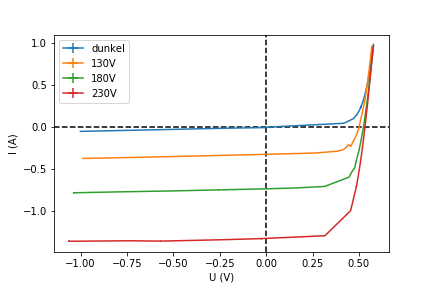
\includegraphics[scale=0.75]{Bilder/UIMono.png}
    \caption{U/I-Kennlinie für das monokristalline Siliziummodul}
    \label{bild:UIMono}
\end{figure}

\begin{figure}[h]
    \centering
    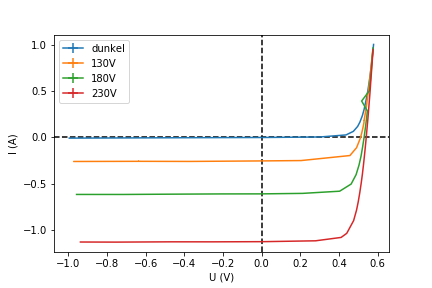
\includegraphics[scale=0.75]{Bilder/UIMulti.png}
    \caption{U/I-Kennlinie für das multikristalline Siliziummodul}
    \label{bild:UIMulti}
\end{figure}

\begin{figure}[h]
    \centering
    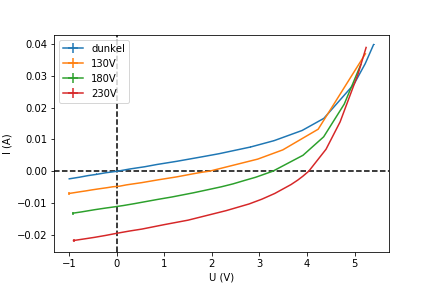
\includegraphics[scale=0.75]{Bilder/UICIS.png}
    \caption{U/I-Kennlinie für das CIS-Modul}
    \label{bild:UICIS}
\end{figure}

Dabei ist der Diodenkennliniencharakter bei den Dunkelmessungen bzw die Verschiebung in negative I-Richtung vor allem bei den 
Siliziumzellen gut zu erkennen. Einzelne Ausreißer, wie z.B. bei der Kennlinie bei $130$V in Abb. \ref{bild:UIMono} oder bei der 
Kennlinie bei $180$V in Abb. \ref{bild:UIMulti}, dürften auf Messfehler zurückzuführen sein. Der Knick im Graphen bei $230$V in Abb.
\ref{bild:UIMono} beruht auf der Unsauberkeit, dass in diesem Messbereich zu wenige Messpunkte gewählt wurden. Dass sich die Kennlinien 
der Dunkelmessung und der Messungen bei eingeschaltetem Licht beim CIS-Modul schneiden, kann daran liegen, dass diese Kennlinie 
nachgemessen wurde und da andere Parameter (Temperatur etc) vorlagen.\\
Beim CIS-Modul ist außerdem der wesentlich flachere Anstieg der Kennlinie auffällig. Hier war während des Versuchs sogar eine reine 
Spannungsregelung möglich. 

